\chapter{Grundlagen}
\label{sec:grundlagen}


\section{Software-Qualität}
\label{sec:softwarequalität}

Nahezu jeder Programmierer ist schon einmal mit dem Begriff der Software-Qualität in Berührung gekommen. Diesen Qualitätsbegriff jedoch genau zu fassen erweist sich als schwierig.
Die DIN-ISO-Norm 9126 definiert Software-Qualität wie folgt:
\\
\glqq Software-Qualität ist die Gesamtheit der Merkmale und Merkmalswerte eines Software-Produkts, die sich auf dessen Eignung beziehen, festgelegte Erforderniss zu erfüllen.\grqq \cite{iso/iec_iso/iec_2001}
\\
Aus dieser Definition wird deutlich, dass es sich bei dem Begriff der Software-Qualität eine multikausale Größe handelt. Das bedeutet, dass zur Bestimmung der Qualität einer Software nicht ein einzelnes Kriterium existiert. Vielmehr verbergen sich hinter dem Begriff eine ganze Reihe verschiedener Kriterien die je nach den gestellten Anforderungen in ihrer Relevanz variieren.\cite[vgl. S.6 ff.]{hoffmann_software-qualitat_2013}
Sammlungen solcher Kriterien werden in sogenannten Qualitätsmodellen zusammengefasst. Die DIN-ISO-Norm 9126 bietet selbst ein solches Qualitätsmodell und definiert damit eine Reihe von wesentlichen Merkmalen, die für die Beurteilung der Software-Qualität eine Rolle spielen. Diese Merkmale sind in der Abbildung \ref{fig:qualitaetsmerkmaleVonSoftwaresystemen} zusammengefasst.
\begin{figure}[htb]
  \centering  
  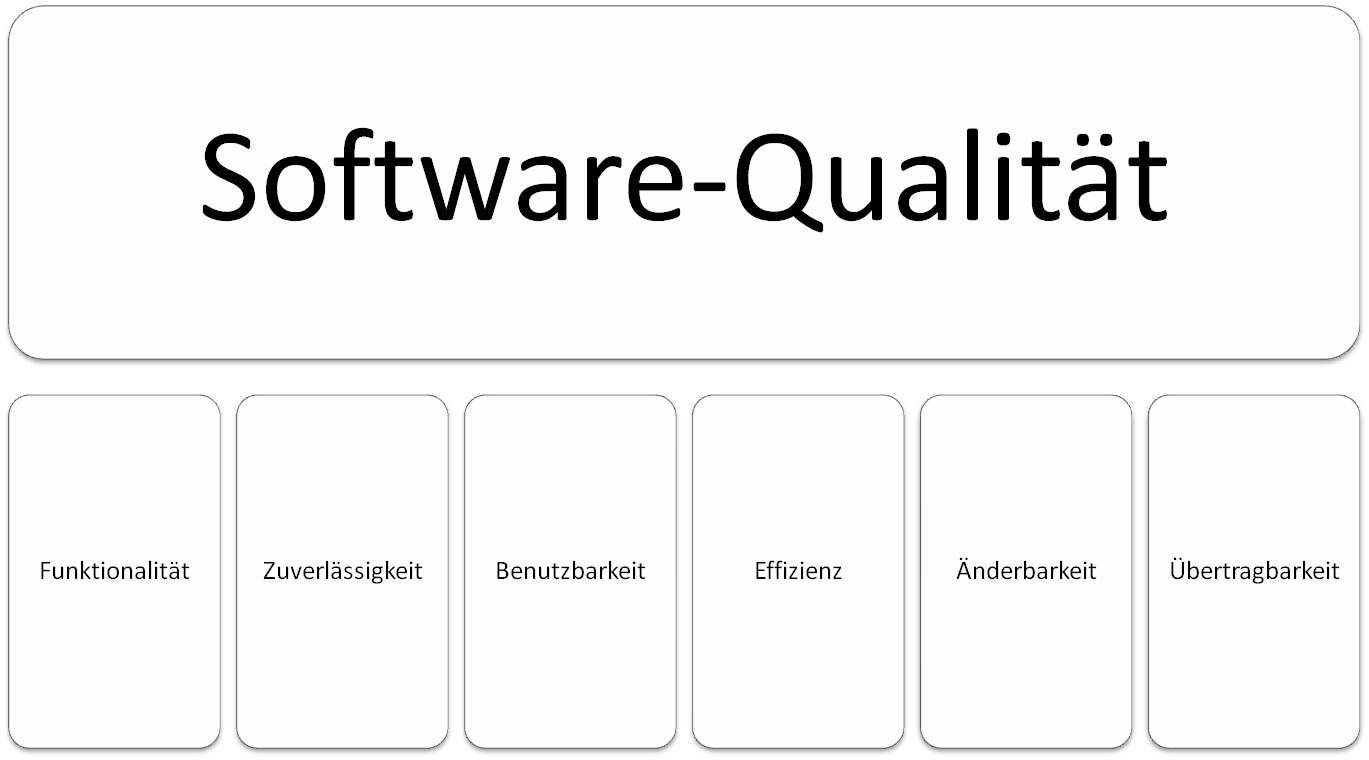
\includegraphics[scale=0.6]{img/softwarequalitaet9126.png}\\
  \footnotesize\sffamily\textbf{Quelle:} \cite{iso/iec_iso/iec_2001}
  \caption{Qualitätsmerkmale von Softwaresystemen (ISO 9126)}
  \label{fig:qualitaetsmerkmaleVonSoftwaresystemen}
\end{figure}
Eine nähere Definition der einzelnen Begriffe des Qualitätsmodells kann beispielsweise dem Buch Software-Qualität von Dirk W. Hoffmann entnommen werden. \cite[S.7 ff.]{hoffmann_software-qualitat_2013}
Um die Qualität einer Software zu Steigern, bietet die moderne Software-Qualitätssicherung eine Vielzahl von Methoden und Techniken.
Ein Teil der Methoden versucht durch eine Verbesserung des Prozesses der Produkterstellung die Entstehung von qualitativ hochwertigen Produkten begünstigt. Diese Methoden fallen in den Bereich der Prozessqualität.
Einen weiteren Bereich bilden die Methoden die zur Verbesserung der  Produktqualität dienen. Bei diesen Methoden wird das Softwareprodukt direkt bezüglich der Qualitätsmerkmale überprüft. Dieser Bereich unterteilt sich in die konstruktive und analytische Qualitätssicherung. \cite[vgl. S.19 ff.]{hoffmann_software-qualitat_2013} Unter konstruktiver Qualitätssicherung versteht man den Einsatz von z.B. Methoden, Werkzeugen oder Standards die
dafür sorgen, dass ein Produkt bestimmte Forderungen erfüllt. 
Unter analytische Qualitätssicherung versteht man den Einsatz von analysierenden bzw. prüfenden Verfahren, die Aussagen
über die Qualität eines Produkts machen. \cite{prof._dr._r._lindermeier_projekt-_2006}
In diesem Bereich der Qualitätssicherung befindet sich unter anderem der klassische Software-Test. Eine Übersicht über das gesamte Gebiet der Software-Qualitätssicherung, wie es sich uns gegenwärtig darstellt, ist in Abbildung \ref{fig:softwareQualitätssicherung} dargestellt. 
\begin{figure}[htb]
  \centering  
  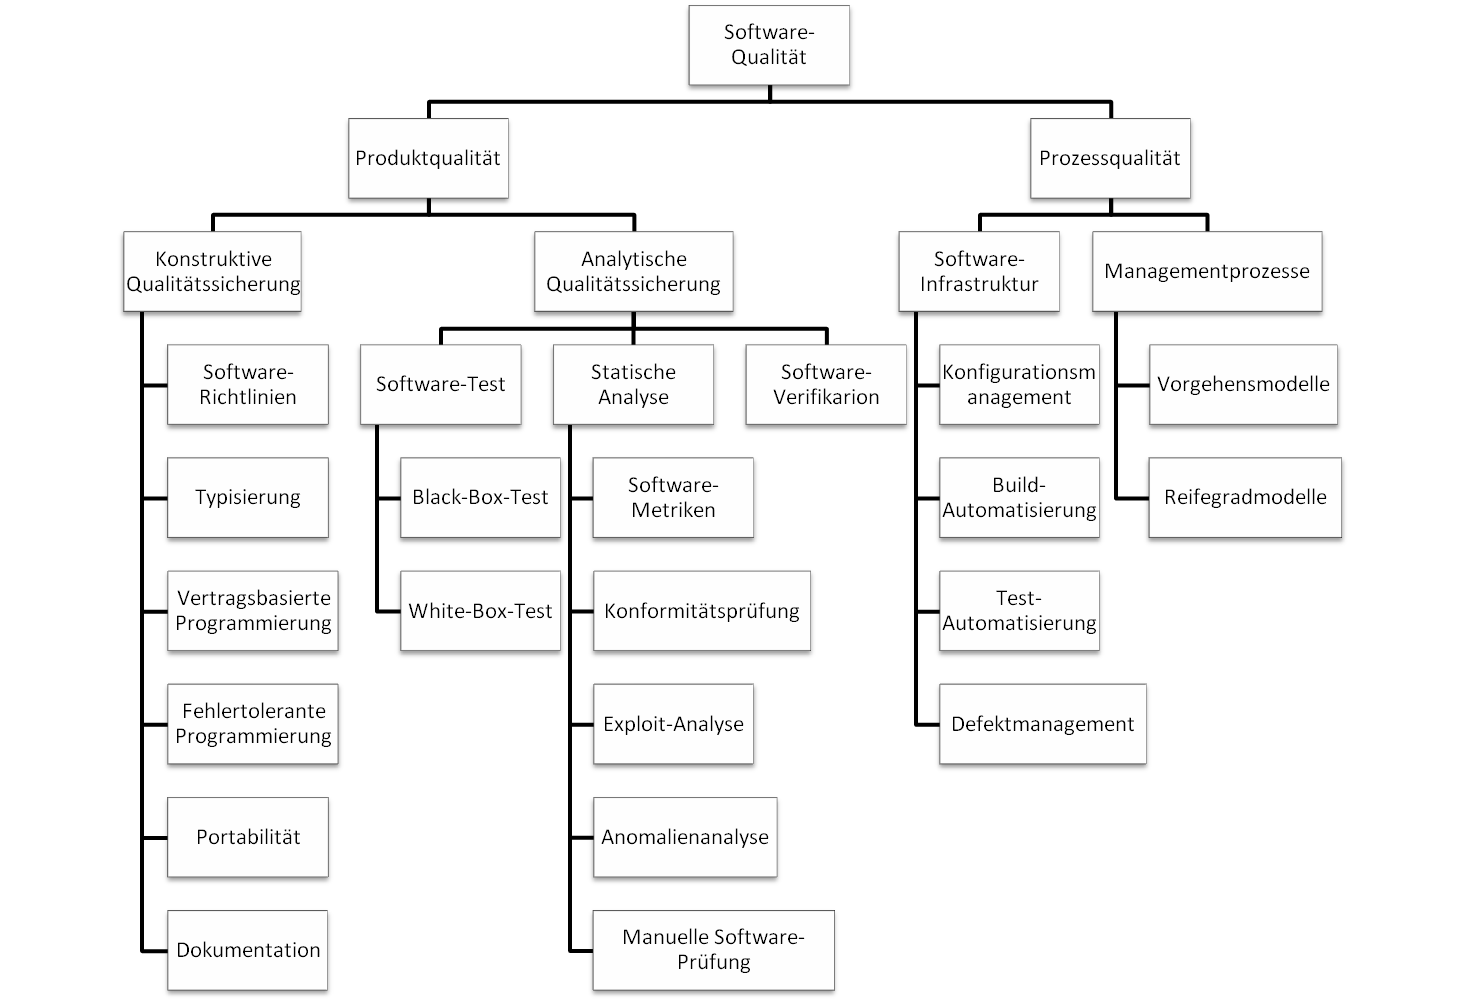
\includegraphics[scale=0.7]{img/softwarequalitaet.png}\\
  \footnotesize\sffamily\textbf{Quelle:} \cite[vgl. S.20]{hoffmann_software-qualitat_2013}
  \caption{Übersicht über das Gebiet der Software-Qualitätssicherung}
  \label{fig:softwareQualitätssicherung}
\end{figure}



\section{Softwaretest}
\label{sec:softwaretest}
Im laufe der Zeit wurden viele Versuche unternommen um die Qualität von Software zu steigern. Besondere Bedeutung hat dabei der Software-Test erlangt.
Der IEEE Std 610.12 definiert den Begriff Test als das ausführen einer Software unter bestimmten Bedingungen mit dem Ziel, die erhaltenen Ergebnisse auszuwerten, also gegen erwartete Werte zu vergleichen.
(Im Original: \glqq An activity in which a system or component is executed under specific conditions, the results are observed or recorded, and an evaluation is made of some aspect of the system or component.\grqq\ \cite{ieee_ieee_1991})
Bereits zu beginn der Softwareentwicklung hat man versucht Programme vor ihrer Auslieferung zu testen. Der dabei erzielte Erfolg entsprach nicht immer den Erwartungen. Im laufe der Jahre wurde das Testen daher auf eine immer breitere Grundlage gestellt. Es entwickelten sich Unterteilungen des Software-Tests die bis heute bestand haben. Hier wären zu nennen:
\begin{itemize}
\item White-Box-Test
\item Black-Box-Test und externe Testgruppe
\item Volume Test, Stress Test und Test auf Systemebene
\end{itemize}
Jeder dieser Begriffe beschreibt bestimmte Techniken, die bei konsequenter Anwendung dazu führen können Fehler in Softwareprodukten zu identifizieren. \cite[vgl. S.18]{thaller_software-test_2002}

Neben der Auswahl der richtigen Techniken für ein bestimmtes Problem spielt in der Praxis die Testkonstruktion eine zentrale Rolle. Bereits für kleine Programme ist es faktisch nicht mehr möglich das Verhalten einer Software für alle möglichen Eingaben zu überprüfen. Es muss sich daher immer auf eine vergleichsweise winzige Auswahl an Testfällen beschränkt werden. Testfälle unterscheiden sich jedoch stark in ihrer Relevanz. Die Auswahl der Testfälle hat daher einen großen Einfluss auf die Anzahl der gefundenen Fahler und damit auch auf die Qualität des Endprodukts. \cite[vgl. S.22]{hoffmann_software-qualitat_2013}

Dennoch ist der Software-Test eines der am meisten verbreiteten Techniken zur Verbesserung der Softwarequalität. Um über lange Sicht gute Software zu produzieren reicht es jedoch nicht aus sich nur auf die Technik des Software-Tests zu stützen. Ein großer Nachteil des Softwaretests ist es, dass Fehler erst in einer relativ späten Phase der Entwicklung identifiziert werden. Je später eine Fehler jedoch erkannt wird, desto teurer wird auch seine Beseitigung. Abbildung \ref{fig:softwareQualitätssicherung} zeigt, dass der Software-Test nur eine von vielen Techniken des Qualitätsmanagement darstellt. Um die Probleme des Software-Tests auszugleichen, ist es daher ratsam, sich bei der Qualitätssicherung möglichst breit aufzustellen und sich nicht nur auf die analytische Qualitätssicherung in Form des Software-Tests zu verlassen. \cite[vgl. S.18]{thaller_software-test_2002}


\section{Testautomatisierung}
\label{sec:testautoGrundlagen}
Das Testen von Software macht in heutigen Projekten einen großen Teil der Projektkosten aus. Studien haben gezeigt, dass das Testen für 50\% 
und mehr der gesamten Projektkosten verantwortlich sein kann. 
Mit Steigender Komplexität der Softwäre steigen diese Kosten immer weiter an. \cite{ramler_economic_2006} \cite{harrold_testing:_2000}
Um diese Kosten zu reduzieren haben sich im laufe der Zeit die bestehenden Testmethoden immer weiter entwickelt und auch neue Ansätze herausgebildet. Einer dieser Ansätze ist es Software-Tests möglichst automatisiert durchzuführen.  \cite{harrold_testing:_2000} Diesen Ansatz fast man mit dem Begriff Testautomatisierung zusammen.
Seidl et al. definieren Testautomatisierung als \glqq die Durchführung von ansonsten manuellen Testtätigkeiten durch Automaten.\grqq \cite[S.7]{seidl_basiswissen_2012}
Diese Definition zeigt, dass das Spektrum der Testautomatisierung breit gefächert ist. Testautomatisierung beschränkt sich nicht nur auf das automatisierte durchführen von Testfällen sondern erstreckt sich über alle Bereiche des Software-Test. [ Die Verschiedenen Möglichkeiten der Testaustomatisierung werden in Kapitel.. dargestellt].
Aus Sicht des Qualitätsmanagement ist die Testautomatisierung sowohl den Methoden zur Steigerung der Produktqualität als auch der Prozessqualität zugeordnet. Ein automatisierter Software-Test hat immer noch den selben Charakter wie ein manueller Software-Test und ist daher ein Teil der analytischen Qualitätssicherung. Allerdings erfordert Testautomatisierung auch immer infrastrukturelle Anpassungen. Automatisierte Testfälle benötigen in der Regel eine Besondere Software-Infrastruktur wie etwa ein Automatisierungsframework. Solche Maßnahmen, die den Programmentwickler aus technischer Sicht in die Lage versetzen, seiner täglichen Arbeit in geregelter und vor allem produktiver Weise nachzugehen, werden den Methoden zur Verbesserung der Prozessqualität zugeordnet. (siehe Abbildung \ref{fig:softwareQualitätssicherung}).
\cite[vgl. Seite 25]{hoffmann_software-qualitat_2013}


\section{Testprozess}
\label{sec:testprozess}

Um Software-Tests effektiv und Strukturiert durchzuführen wird eine verfeinerter Ablaufplan für die einzelnen Testaufgaben benötigt. Diesen Ablaufplan fassen Splinner und Linz im fundamentalen Testprozess zusammen. Die einzelnen Arbeitsschritte die im Lebenszyklus eines Software-Tests anfallen werden dabei verschiedenen Phasen zugeordnet.
Durch den Testprozess wird die Aufgabe des Testens so in kleinere Testaufgaben untergliedert.

Testaufgaben, die man dabei unterscheidet sind:

\begin{itemize}
	  \itemsep0pt
      \item Testplanung und Steuerung
      \item Testanalyse und Testdesign
      \item Testrealisierung und Testdurchführung
      \item Testauswertung und Bericht
      \item Abschluss der Testaktivitäten       
\end{itemize}

\glqq Obgleich die Aufgaben in sequenzieller Reihenfolge im Testprozess angegeben sind, können sie sich überschneiden und teilweise auch gleichzeitig durchgeführt werden.\grqq\ \cite[S.19]{spillner_basiswissen_2007} Auf Grundlage des fundamentalen Testprozesses nach Splinner und Linz werden im folgenden diese Teilaufgaben näher beschrieben. \cite[S.20ff]{spillner_basiswissen_2007}
Diese Beschreibung wird durch Ausführungen von Seidl et al. erweitert. \cite[Seite 9 ff.]{seidl_basiswissen_2012}

\subsection{Testplanung und Steuerung}
\label{subsec:testplanung_und_steuerung}
Um dem Umfang und der Komplexität heutiger Software-Tests gerecht zu werden, benötigt man zu Beginn des Testprozesses eine genaue Planung.
Ziel dieser Planung ist es, den Rahmen für die weiteren Testaktivitäten festzulegen. Die Aufgaben und die Zielsetzungen der Tests müssen ermittelt wurden. Eine Ressourcenplanung wird benötigt und eine geeignete Teststrategie muss ermittelt werden. In Kapitel \ref{sec:softwaretest} wurde bereits erwähnt, dass das vollständige Testen einer Anwendung in der Regel nicht möglich ist. Die einzelnen Systemteile müssen daher nach Schwere der zu erwartenden Fehlerwirkung priorisiert werden. Um so schwerwiegender die zu erwartende Fehlerwirkung ist, umso intensiver muss der betrachtete Systemteil auch getestet werden. Ziel der Teststrategie ist also \glqq die optimale Verteilung der Tests auf die \frqq richtigen\flqq\ Stellen das Softwaresystems.\grqq\ \cite[S.21]{spillner_basiswissen_2007} Steht das Softwareprojekt unter einem hohen Zeitdruck müssen Testfälle zusätzlich Priorisiert werden.
Um zu verhindern, dass das Testen zu einem endlosen Prozess wird, müssen auch geeignete Testendekriterien festgelegt werden. Anhand dieser Kriterien kann später entschieden werden ob der Testprozess abgeschlossen werden kann.

Bereits zu Beginn des Testprozesses werden auch wichtige Grundsteine für eine spätere Testautomatisierung gelegt. Es muss entschieden werden, in welchen Teststufen und Testbereichen eine Automatisierung eingesetzt werden soll. Vor allem ist die frage zu klären ob und in welchem Ausmaß eine Automatisierung überhaupt sinnvoll ist.
Entscheidet man sich für eine Testautomatisierung hat das in der Regel große Auswirkung auf die einzusetzenden Ressourcen und die Zeitliche Planung und Aufwandsschätzung.
Oftmals wird im Rahmen der Tests eine besondere Werkzeugunterstützung oder Infrastruktur benötigt. Derartige Punkte müssen auch bereits in der frühen Planungsphase berücksichtigt werden. Wie Kapitel \ref{sec:softwaretest} gezeigt hat, ist das im besonderen der Fall wenn in der Planung beschlossen wird, dass die Testfälle automatisiert durchgeführt werden sollen.

Die Gesamten erarbeiteten Rahmenbedingungen werden in einem Testkonzept dokumentiert.
Eine mögliche Vorlage für dieses Dokument bietet die internationale Norm IEEE 829-2008 \cite{ieee_ieee_2008}.
Neben der frühzeitigen Planung der Tests muss während des gesamten Testprozesses eine Steuerung erfolgen.
Hierfür werden die Ergebnisse und Fortschritte der Tests und des Projekts laufend erhoben, geprüft und bewertet. Werden Probleme erkannt, kann so rechtzeitig gegengesteuert werden. 

\subsection{Testanalyse und Testdesign}
\label{subsec:testanalyse_und_design}
In dieser Phase wird zunächst die Qualität der Testbasis überprüft. Alle Dokumente die für die Erstellung der Testfälle benötigt werden müssen in ausreichendem Detailgrad vorhanden sind. Mit Hilfe der qualitätsgesicherten Dokumente kann die eigentliche Testfallerstellung beginnen.
Anhand der Informationen aus dem Testkonzept und den Spezifikationen werden mittels strukturierter Testfallerstellungsmethoden logische Testfälle erstellt. Diese logischen Testfälle können dann in einer späteren Phase konkretisiert werden, indem ihnen z.B. tatsächliche Eingabewerte zugeordnet werden. Für jeden dieser Testfälle müssen die möglichen Rand- und Vorbedingungen so wie ein erwartetes Ergebnis bestimmt werden. 
In dieser Phase beginnt auch die Umsetzung der Testfälle in der Testautomatisierung.
Abgestimmt auf die ausgewählten Automatisierungswerkzeuge und die zu testende Software  muss die Umgebung für die Testautomatisierung vorbereitet werden. Anhand der Vorgaben des Testkonzeptes können dann jene Testfälle und Testabläufe ausgewählt werden die im Zuge der Testautomatisierung implementiert werden sollen. Hierbei wird noch einmal die technische Umsetzbarkeit der ausgewählten Testfälle geprüft. Bei der Auswahl der Testfälle sollte zu beginn eine möglichst breite Testabdeckung angestrebt werden.
Problemfelder können dann später durch weitere Testfälle in in der Tiefe getestet werden.

\subsection{Testrealisierung und Testdurchführung}
\label{subsec:testrealisierung_und_durchführung}
In diesem Schritt des Testprozesses werden aus den Logischen Testfällen der vorangegangenen Phase konkrete Testfälle gebildet.
Diese Testfälle werden anhand ihrer fachlichen und technischen Zusammengehörigkeit zu Testszenarien gruppiert und anhand der Vorgaben aus dem Testkonzept priorisiert.
Sobald die zu testende Software zur Verfügung steht, kann mit der Abarbeitung der Testfälle begonnen werden. Die dabei erhaltenen Ergebnisse werden vollständig protokolliert. Werden im Zuge der Durchführung Fehler aufgedeckt, muss darauf in geeigneter Weise reagiert werden. Es könnte beispielsweise ein zuvor definierter Fehlerprozess gestartet werden.
Korrekturen und nachgehende Veränderungen am Testobjekt werden durch eine Wiederholung der Testläufe abgedeckt.
Aus Sicht der Testautomatisierung beginnt in dieser Phase die technische Umsetzung der Testfälle.
In vielen Fällen bedeutet das Programmiertätigkeit. Diese Programmiertätigkeiten sind wiederum anfällig für eigene Fehler und müssen daher in angemessener Weise qualitätsgesichert werden. Auch bei der Testautomatisierung ist eine Zusammenfassung von Testfällen sinnvoll. Auf diese weise kann man funktionalen und logischen Abhängigkeiten zwischen den Testfällen gerecht werden.
Nach der Implementierung können die geplanten Testfälle durchgeführt werden.
Gerade bei der Automatisierung ist eine genaue Protokollierung der Ergebnisse besonders wichtig.
Nur dadurch ist es später möglich, aufgetretene Fehler überhaupt zu lokalisieren.


\subsection{Testauswertung und Bericht}
\label{subsec:testauswertung_und_bericht}
In dieser Phase des Prozesses wird geprüft, ob die im Testkonzept definierten Testendekriterien erreicht wurden. Sind alle Forderungen erfüllt, kann es zu einem Abschluss der Testaktivitäten kommen. Kommt es zu Abweichungen im Bezug auf diese Kriterien, muss darauf entsprechend reagiert werden. Es können Fehlerkorrekturen durchgeführt werden oder neue Testfälle erstellt werden. Aber auch der umgekehrte Fall ist möglich. Es kann dazu kommen, dass Endekriterien nur mit unverhältnismäßig hohem Aufwand erreicht werden 
und daher bestimmte Testfälle entfallen oder Kriterien überdacht werden müssen.

Für die Testautomatisierung ist wesentliche Aufgabe dieser Phase die Auswertung und Aufarbeitung der erhaltenen Ergebnisse. Automatisierte Tests generieren oftmals eine Fülle an Log-Dateien und Protokollen. Um aus diesen Ergebnissen die richtigen Schlüsse zu ziehen und sie für dritte zugänglich zu machen müssen sie in eine lesbare Form gebracht werden.

In jedem Fall muss über die erhaltenen Ergebnisse und das daraus resultierende Vorgehen ein Testbericht erstellt werden. Je nach Umfang und Phase der Test kann dieser mehr oder weniger formal ausfallen. Für einen Komponententests reicht beispielsweise eine formlose Mitteilung. Höhere Teststufen erfordern allerdings einen formaleren Bericht.



\subsection{Abschluss der Testaktivitäten}
\label{subsec:abschluss_der_testaktivitäten}
Sind die Testaktivitäten abgeschlossen sollten zum Schluss alle im laufe des Testprozesses gemachten Erfahrungen analysiert werden. So können die gewonnenen Erkenntnisse für spätere Projekte genutzt werden. Dadurch kann eine stetige Verbesserung des Testprozesses erreicht werden.
Die während des Prozesses erstellte Testware sollte archiviert werden. Auf diese weise steht sie für folgende Regressionstests zur Verfügung. Die Kosten in Wartung und Pflege der Software können damit gesenkt werden.
Bei der Testautomatisierung bedeutet das, die Wiederverstellbarkeit der Testumgebung und des Sourcecodes der Tests sicherzustellen.
\newline\\
Abschließend ist zu sagen, dass sich die Testautomatisierung in der Regel gut in einen bereits bestehenden Testprozess integrieren lasst. Sie wird allerdings \glqq den Prozess nicht verbessern oder gerade richten, sondern nur unterstützen.\grqq\ \cite[S.21]{seidl_basiswissen_2012} Ist der Testprozess schon vor einführung einer Automatisierung schlecht gelaufen, wird er es nach der Einführung auch noch.
Die Testautomatisierung ist also nicht als Heilmittel für schlecht laufende Prozesse gedacht sondern als Möglichkeit sich einen bereits gut laufenden Prozess effizienter zu gestalten.

\section{Vorgehensmodelle}
\label{sec:vorgehensmodelle}
Der in Kapitel \ref{sec:testprozess} beschriebene Testprozess ist nicht als losgelöster, eigenständiger Prozess zu betrachten. Vielmehr ist der Testprozess immer ein Teil eines größeren Entwicklungsablaufes bei der Erstellung eines Softwareprodukts. Einen solchen Entwicklungsablauf versucht man mit Hilfe von sogenannten Softwareentwicklungsmodellen, auch Vorgehensmodelle genannt, abzubilden.
Ein Projekt wird dazu in einzelne Phasen untergliedert an deren Ende ein gewisses Ziel bzw. Ergebnis steht.
Auf gröbster ebene können dabei vier Hauptphasen unterschieden werden, die auch so von Seidl et al. verwendet werden \cite[S.21 ff.]{seidl_basiswissen_2012}. Diese Phasen finden sich mehr oder weniger Ausgeprägt in den meisten der gängigen Vorgehensmodelle wieder:

\begin{itemize}
\item Spezifikation
\item Design
\item Entwicklung
\item Test
\end{itemize}

Das Testen, bzw. der Testprozess ist also eine von mehreren Phasen in solch einem Entwicklungsmodell.
Es gibt eine Vielzahl von unterschiedlichen Softwareentwicklungsmodellen. Der Hauptunterschied liegt meist in der zeitlichen Koppelung und der inhaltlichen Ausprägung der einzelnen Phasen. Die einzelnen Phasen können sich innerhalb eines Vorgehensmodells überschneiden und wiederholen und müssen auch nicht immer wie in der Auflistung angegeben sequentiell abgearbeitet werden.
Aus der Sicht der Testautomatisierung ist daher eine Einteilung der verschiedenen Vorgehensmodelle in zwei Gruppen sinnvoll: \cite[vgl. S.21 ff.]{seidl_basiswissen_2012}

\begin{itemize}
\item Klassische Entwicklungsmodelle, die eher sequentiell ausgerichtet sind
\item Iterative und agile Entwicklungsmodelle, die sich durch Parallelisierung und kurze Iterationen auszeichnen.
\end{itemize}

\subsection{Klassische Entwicklungsmodelle}
\label{subsec:klassische_entwicklungsmodelle}

\begin{figure}[htb]
  \centering  
  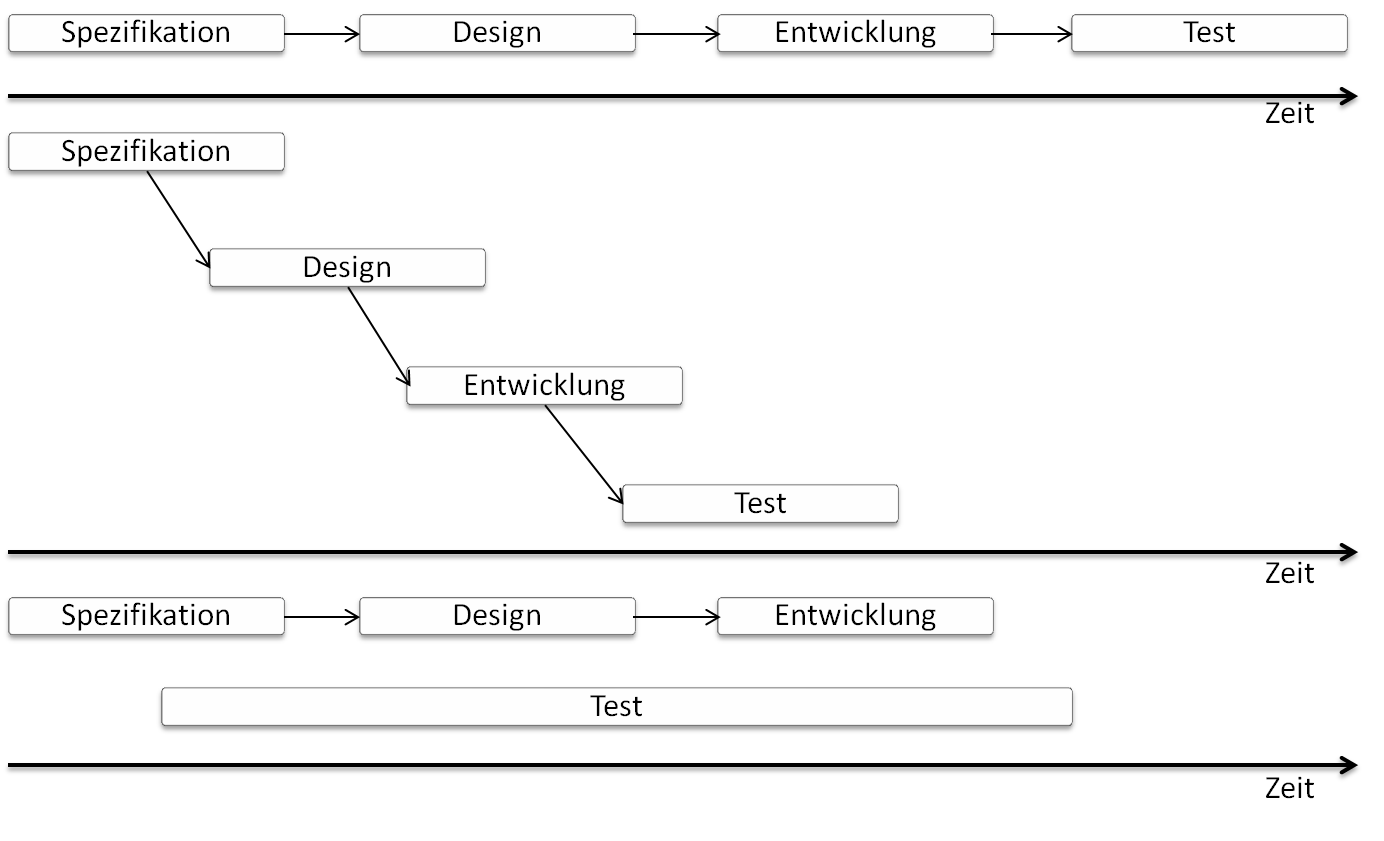
\includegraphics[scale=0.7]{img/sequentielleentwicklungsmodelle.png}\\
  \footnotesize\sffamily\textbf{Quelle:} \cite[vgl. S.22]{seidl_basiswissen_2012}
  \caption{Verschiedene Ausprägungen klassischer Entwicklungsmodelle}
  \label{fig:verschiedene_auspraegungen_klassischer_entwicklungsmodelle}
\end{figure}

\subsection{Iterative und agile Entwicklungsmodelle}
\label{subsec:iterative_und_agile_entwicklungsmodelle}

\begin{figure}[htb]
  \centering  
  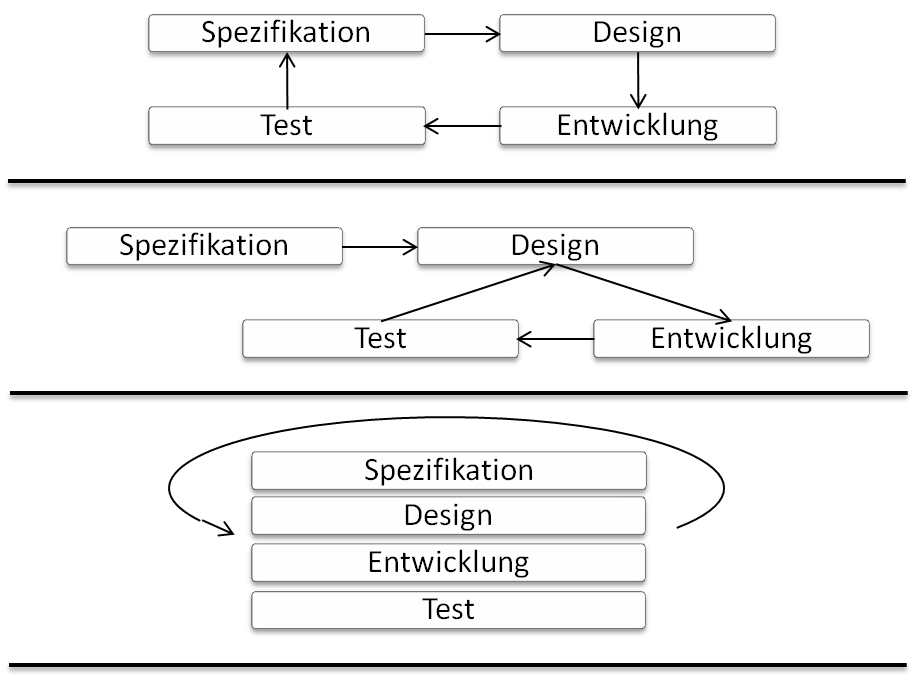
\includegraphics[scale=0.7]{img/iterativeentwicklungsmodelle.png}\\
  \footnotesize\sffamily\textbf{Quelle:} \cite[vgl. S.24]{seidl_basiswissen_2012}
  \caption{Verschiedene Ausprägungen iterativer und agiler Entwicklungsmodelle}
  \label{fig:verschiedene_auspraegungen_iterativer_und_agiler_entwicklungsmodelle}
\end{figure}

